\documentclass{article}

% if you need to pass options to natbib, use, e.g.:
% \PassOptionsToPackage{numbers, compress}{natbib}
% before loading nips_2018

% ready for submission
\usepackage[preprint]{nips_2018}

% to compile a preprint version, e.g., for submission to arXiv, add
% add the [preprint] option:
% \usepackage[preprint]{nips_2018}

% to compile a camera-ready version, add the [final] option, e.g.:
% \usepackage[final]{nips_2018}

% to avoid loading the natbib package, add option nonatbib:
% \usepackage[nonatbib]{nips_2018}

\usepackage[utf8]{inputenc} % allow utf-8 input
\usepackage[T1]{fontenc}    % use 8-bit T1 fonts
\usepackage{hyperref}       % hyperlinks
\usepackage{url}            % simple URL typesetting
\usepackage{booktabs}       % professional-quality tables
\usepackage{amsfonts}       % blackboard math symbols
\usepackage{nicefrac}       % compact symbols for 1/2, etc.
\usepackage{microtype}      % microtypography
\usepackage{graphicx} %Loading the package
\graphicspath{{figures/}}

\title{Seeking Methods to Improve Small Object Detection}

% The \author macro works with any number of authors. There are two
% commands used to separate the names and addresses of multiple
% authors: \And and \AND.
%
% Using \And between authors leaves it to LaTeX to determine where to
% break the lines. Using \AND forces a line break at that point. So,
% if LaTeX puts 3 of 4 authors names on the first line, and the last
% on the second line, try using \AND instead of \And before the third
% author name.

\author{
  Shiming Luo\thanks{Use footnote ---\emph{not} for} \\
  Department of Computer Science\\
  University of California, San Diego\\
  9500 Gilman Drive, La Jolla, CA 92093\\
  \texttt{shl666@eng.ucsd.edu} \\
  %% examples of more authors
  \And
  Yu Zhong \\
  Department of Computer Science \\
  University of California, San Diego \\
  9500 Gilman Drive, La Jolla, CA 92093\\
  \texttt{yuz871@eng.ucsd.edu} \\
}

\begin{document}
% \nipsfinalcopy is no longer used

\maketitle

\begin{abstract}
  The following paper discusses several attempts, including enlargement of receptive 
  field, specific data augmentation, and anchor boxes refinement to increase the confidence
  level of detecting small objects in one picture, especially human being detection
  and faces detection. Throughout the entire experiment, reasoning of different
  methodologies and results are provided in the following sections.
\end{abstract}

\section{Introduction}

\subsection{Motivation}
Given the history of computer vision, machine learning has become one of the most popular 
approaches to achieve solutions to different vision-related tasks included image classification, 
object detection, video motion tracking, super resolution, and style transfer. In the field of object 
detection, multiple neural network based solutions have been widely accepted and applied in many 
situations with increasing speed and accuracy. Given the need for higher accuracy, experimenters 
decide to further improve the accuracy on objection detection, especially on small objects detection.

\subsection{Overview}

\subsubsection{History}

Apply instant object detection has always been one of the goals of computer vision. Starting from 1970s, researchers had been researched into human vision and discovered a series of connections between neuroscience and vision system. Therefore, theories such as primal sketches had attracted enough academic attention and early computer vision started around 1970s. Later, feature-base methods such as using pose consistency(also called alignment), and other geometry primitives to analyze images and extract features. in 1990s, sliding window approaches was among one of the most popular way to recognize human faces. Meanwhile, appearance-based methods also showed potentials in mimicking biological vision system and can be therefore a key method in machine vision. Instead of early canny edge detection technique, features of an image now include more and more features and thus the variety of feature matching became heated again. In early 2000s, local features were utilized in recognition for object instances and then bag of features model prevailed, while in the same time, new features description such as scale-invariant feature transform (SIFT) and histogram of oriented gradients became some of the most common feature description until the era of machine learning. In the recent decade, application of convolution neural network based studies became the most popular topic in computer vision field and most studies were directly related to techniques or methodologies depended on deep learning. Given the huge success brought by the introduction of neural network, most vision tasks apply the methodology of end-to-end learning with significant amount of training data. 

Provided the successful object classification network, it was reasonable to naively extract all possible bounding boxes in one image and classify each of them to select the one with highest confidence level. However, such algorithm was not practical based on hardware capabilities. Hence, the bounding problem was abstracted into a regression problem and later became a learnable process. Early attempts such as Overfeat did show promising results in tasks combining classification and localization.
As more comprehensive datasets such PASCAL, ILSVRC, MSCOCO were available for researchers, training and testing became more convenient and thus more time could be devoted onto discovery of new models. Region proposals became the most promising method to solve bounding box issue in detection. However, its repetition of computing features slowed down the training process and therefore new algorithm and learning procedure were then invented to greatly improve the speed of region-based convolutional neural network. In year 2016, proposal-free object detection pipeline was invented and named "You Only Look Once." (YOLO) Such procedure include default boxes prediction on given number of cells and results were surprisingly fast. At the same year, the Single Shot Multibox Detector was invented and combined "Look Once" idea from YOLO and anchor boxes from Faster R-CNN and made such algorithm one of the fastest object detection algorithm so far.

\subsubsection{Issue}

Due to the fact that object detection network often apply artificial neural network, in which convolution and pooling are fundamental operations of neural network, the tensor height and width will shrink continuously during those operations, and therefore expand the receptive field in tensors corresponding to the original dimension in the input image. Consequently, if objects appear small in the input image, the detection network may neglect or yield a marginal confidence level for such object. Therefore, researchers would like to seek a possible method to increase the confidence level in small object detection. 

\section{Experiment Proposals}

Based on the given code base, the SSD algorithm is implemented through addition of layers upon VGG network, one of the most popular classification network invented in year 2014. The code transforms the final fully connected layer into additional convolutional layers with no dropout layer. For bounding box prediction, author extracts different features in between different convolutional layers. Based on the dimension of feature map and precalculated anchor sizes, anchor boxes are projected back to the original picture and bounding boxes and prediction are made. Such methodology greatly enhances the small object detection, which is to some extent compromised in YOLO structure. Based on the aforementioned chain of thoughts, we researchers intend to further enhance the confidence level of small object detection by the following various experiments.

\subsection{Advancing Feature Maps to Early Layers}

After multiple layers of convolution and pooling, the dimensions of the feature maps that are used for anchor box prediction are $38 \times 38, 19 \times 19, 10 \times 10, 5 \times 5, 3 \times 3, 1 \times 1 $. In this project, the effects of advancing feature maps to earlier block, for example, using an early feature map in between VGG with a dimension of $150 \times 150$ or $75 \times 75$ will be discussed later in the report.

\begin{figure}
	\centering
	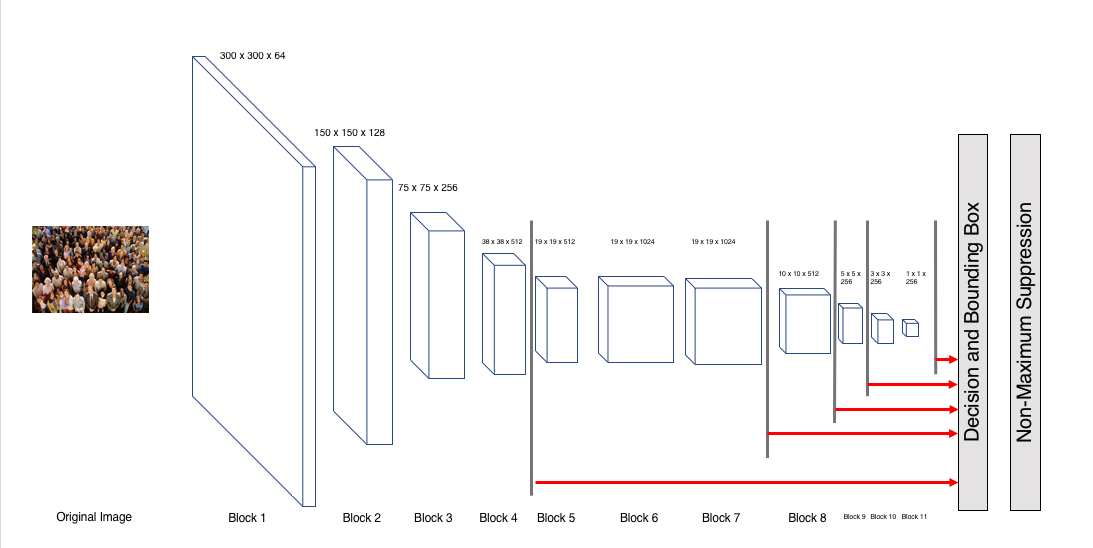
\includegraphics[height=7cm]{VGGSSDOriginal.png}
	\caption{Convolution Neural Network with Fully Connected Layer but no Batch Normalization}	
	\label{F1}
	\end{figure}


\subsection{Addition of Anchor Boxes}

The default anchor boxes set include 6 predetermined anchor sizes and aspect ratios, which was hypothesized and tested extensively by researchers. In addition to advance feature maps to early layers, insertion of another anchor box set may affect the final result as well. The results will be discussed in the later section.

\subsection{Training Set Variation}

To further exploit the structure of VGG-based neural network to realize small object detection, researchers focus on a binary human faces recognition due to the availability of human faces datasets. Therefore, instead of PASCAL VOC 2007 dataset, experimenters apply the WIDER FACE dataset to verify the effects of small object detection. 

\subsection{Input Image Processing}

Given the high speed of object detection by SSD, researchers also experiment on the trade-off between speed and accuracy to improve small faces detection. Cropping the images into sections and send cropped and rescaled images into the network to achieve the final results.



The \LaTeX{} style file contains three optional arguments: \verb+final+,
which creates a camera-ready copy, \verb+preprint+, which creates a
preprint for submission to, e.g., arXiv, and \verb+nonatbib+, which will
not load the \verb+natbib+ package for you in case of package clash.

\paragraph{New preprint option for 2018}
If you wish to post a preprint of your work online, e.g., on arXiv,
using the NIPS style, please use the \verb+preprint+ option. This will
create a nonanonymized version of your work with the text
``Preprint. Work in progress.''  in the footer. This version may be
distributed as you see fit. Please \textbf{do not} use the
\verb+final+ option, which should \textbf{only} be used for papers
accepted to NIPS.

At submission time, please omit the \verb+final+ and \verb+preprint+
options. This will anonymize your submission and add line numbers to aid
review. Please do \emph{not} refer to these line numbers in your paper
as they will be removed during generation of camera-ready copies.

The file \verb+nips_2018.tex+ may be used as a ``shell'' for writing
your paper. All you have to do is replace the author, title, abstract,
and text of the paper with your own.

The formatting instructions contained in these style files are
summarized in Sections \ref{gen_inst}, \ref{headings}, and
\ref{others} below.

\section{General formatting instructions}
\label{gen_inst}

The text must be confined within a rectangle 5.5~inches (33~picas)
wide and 9~inches (54~picas) long. The left margin is 1.5~inch
(9~picas).  Use 10~point type with a vertical spacing (leading) of
11~points.  Times New Roman is the preferred typeface throughout, and
will be selected for you by default.  Paragraphs are separated by
\nicefrac{1}{2}~line space (5.5 points), with no indentation.

The paper title should be 17~point, initial caps/lower case, bold,
centered between two horizontal rules. The top rule should be 4~points
thick and the bottom rule should be 1~point thick. Allow
\nicefrac{1}{4}~inch space above and below the title to rules. All
pages should start at 1~inch (6~picas) from the top of the page.

For the final version, authors' names are set in boldface, and each
name is centered above the corresponding address. The lead author's
name is to be listed first (left-most), and the co-authors' names (if
different address) are set to follow. If there is only one co-author,
list both author and co-author side by side.

Please pay special attention to the instructions in Section \ref{others}
regarding figures, tables, acknowledgments, and references.

\section{Headings: first level}
\label{headings}

All headings should be lower case (except for first word and proper
nouns), flush left, and bold.

First-level headings should be in 12-point type.

\subsection{Headings: second level}

Second-level headings should be in 10-point type.

\subsubsection{Headings: third level}

Third-level headings should be in 10-point type.

\paragraph{Paragraphs}

There is also a \verb+\paragraph+ command available, which sets the
heading in bold, flush left, and inline with the text, with the
heading followed by 1\,em of space.

\section{Citations, figures, tables, references}
\label{others}

These instructions apply to everyone.

\subsection{Citations within the text}

The \verb+natbib+ package will be loaded for you by default.
Citations may be author/year or numeric, as long as you maintain
internal consistency.  As to the format of the references themselves,
any style is acceptable as long as it is used consistently.

The documentation for \verb+natbib+ may be found at
\begin{center}
  \url{http://mirrors.ctan.org/macros/latex/contrib/natbib/natnotes.pdf}
\end{center}
Of note is the command \verb+\citet+, which produces citations
appropriate for use in inline text.  For example,
\begin{verbatim}
   \citet{hasselmo} investigated\dots
\end{verbatim}
produces
\begin{quote}
  Hasselmo, et al.\ (1995) investigated\dots
\end{quote}

If you wish to load the \verb+natbib+ package with options, you may
add the following before loading the \verb+nips_2018+ package:
\begin{verbatim}
   \PassOptionsToPackage{options}{natbib}
\end{verbatim}

If \verb+natbib+ clashes with another package you load, you can add
the optional argument \verb+nonatbib+ when loading the style file:
\begin{verbatim}
   \usepackage[nonatbib]{nips_2018}
\end{verbatim}

As submission is double blind, refer to your own published work in the
third person. That is, use ``In the previous work of Jones et
al.\ [4],'' not ``In our previous work [4].'' If you cite your other
papers that are not widely available (e.g., a journal paper under
review), use anonymous author names in the citation, e.g., an author
of the form ``A.\ Anonymous.''

\subsection{Footnotes}

Footnotes should be used sparingly.  If you do require a footnote,
indicate footnotes with a number\footnote{Sample of the first
  footnote.} in the text. Place the footnotes at the bottom of the
page on which they appear.  Precede the footnote with a horizontal
rule of 2~inches (12~picas).

Note that footnotes are properly typeset \emph{after} punctuation
marks.\footnote{As in this example.}

\subsection{Figures}

\begin{figure}
  \centering
  \fbox{\rule[-.5cm]{0cm}{4cm} \rule[-.5cm]{4cm}{0cm}}
  \caption{Sample figure caption.}
\end{figure}

All artwork must be neat, clean, and legible. Lines should be dark
enough for purposes of reproduction. The figure number and caption
always appear after the figure. Place one line space before the figure
caption and one line space after the figure. The figure caption should
be lower case (except for first word and proper nouns); figures are
numbered consecutively.

You may use color figures.  However, it is best for the figure
captions and the paper body to be legible if the paper is printed in
either black/white or in color.

\subsection{Tables}

All tables must be centered, neat, clean and legible.  The table
number and title always appear before the table.  See
Table~\ref{sample-table}.

Place one line space before the table title, one line space after the
table title, and one line space after the table. The table title must
be lower case (except for first word and proper nouns); tables are
numbered consecutively.

Note that publication-quality tables \emph{do not contain vertical
  rules.} We strongly suggest the use of the \verb+booktabs+ package,
which allows for typesetting high-quality, professional tables:
\begin{center}
  \url{https://www.ctan.org/pkg/booktabs}
\end{center}
This package was used to typeset Table~\ref{sample-table}.

\begin{table}
  \caption{Sample table title}
  \label{sample-table}
  \centering
  \begin{tabular}{lll}
    \toprule
    \multicolumn{2}{c}{Part}                   \\
    \cmidrule(r){1-2}
    Name     & Description     & Size ($\mu$m) \\
    \midrule
    Dendrite & Input terminal  & $\sim$100     \\
    Axon     & Output terminal & $\sim$10      \\
    Soma     & Cell body       & up to $10^6$  \\
    \bottomrule
  \end{tabular}
\end{table}

\section{Final instructions}

Do not change any aspects of the formatting parameters in the style
files.  In particular, do not modify the width or length of the
rectangle the text should fit into, and do not change font sizes
(except perhaps in the \textbf{References} section; see below). Please
note that pages should be numbered.

\section{Preparing PDF files}

Please prepare submission files with paper size ``US Letter,'' and
not, for example, ``A4.''

Fonts were the main cause of problems in the past years. Your PDF file
must only contain Type 1 or Embedded TrueType fonts. Here are a few
instructions to achieve this.

\begin{itemize}

\item You should directly generate PDF files using \verb+pdflatex+.

\item You can check which fonts a PDF files uses.  In Acrobat Reader,
  select the menu Files$>$Document Properties$>$Fonts and select Show
  All Fonts. You can also use the program \verb+pdffonts+ which comes
  with \verb+xpdf+ and is available out-of-the-box on most Linux
  machines.

\item The IEEE has recommendations for generating PDF files whose
  fonts are also acceptable for NIPS. Please see
  \url{http://www.emfield.org/icuwb2010/downloads/IEEE-PDF-SpecV32.pdf}

\item \verb+xfig+ "patterned" shapes are implemented with bitmap
  fonts.  Use "solid" shapes instead.

\item The \verb+\bbold+ package almost always uses bitmap fonts.  You
  should use the equivalent AMS Fonts:
\begin{verbatim}
   \usepackage{amsfonts}
\end{verbatim}
followed by, e.g., \verb+\mathbb{R}+, \verb+\mathbb{N}+, or
\verb+\mathbb{C}+ for $\mathbb{R}$, $\mathbb{N}$ or $\mathbb{C}$.  You
can also use the following workaround for reals, natural and complex:
\begin{verbatim}
   \newcommand{\RR}{I\!\!R} %real numbers
   \newcommand{\Nat}{I\!\!N} %natural numbers
   \newcommand{\CC}{I\!\!\!\!C} %complex numbers
\end{verbatim}
Note that \verb+amsfonts+ is automatically loaded by the
\verb+amssymb+ package.

\end{itemize}

If your file contains type 3 fonts or non embedded TrueType fonts, we
will ask you to fix it.

\subsection{Margins in \LaTeX{}}

Most of the margin problems come from figures positioned by hand using
\verb+\special+ or other commands. We suggest using the command
\verb+\includegraphics+ from the \verb+graphicx+ package. Always
specify the figure width as a multiple of the line width as in the
example below:
\begin{verbatim}
   \usepackage[pdftex]{graphicx} ...
   \includegraphics[width=0.8\linewidth]{myfile.pdf}
\end{verbatim}
See Section 4.4 in the graphics bundle documentation
(\url{http://mirrors.ctan.org/macros/latex/required/graphics/grfguide.pdf})

A number of width problems arise when \LaTeX{} cannot properly
hyphenate a line. Please give LaTeX hyphenation hints using the
\verb+\-+ command when necessary.

\subsubsection*{Acknowledgments}

Use unnumbered third level headings for the acknowledgments. All
acknowledgments go at the end of the paper. Do not include
acknowledgments in the anonymized submission, only in the final paper.

\section*{References}

References follow the acknowledgments. Use unnumbered first-level
heading for the references. Any choice of citation style is acceptable
as long as you are consistent. It is permissible to reduce the font
size to \verb+small+ (9 point) when listing the references. {\bf
  Remember that you can use more than eight pages as long as the
  additional pages contain \emph{only} cited references.}
\medskip

\small

[1] Alexander, J.A.\ \& Mozer, M.C.\ (1995) Template-based algorithms
for connectionist rule extraction. In G.\ Tesauro, D.S.\ Touretzky and
T.K.\ Leen (eds.), {\it Advances in Neural Information Processing
  Systems 7}, pp.\ 609--616. Cambridge, MA: MIT Press.

[2] Bower, J.M.\ \& Beeman, D.\ (1995) {\it The Book of GENESIS:
  Exploring Realistic Neural Models with the GEneral NEural SImulation
  System.}  New York: TELOS/Springer--Verlag.

[3] Hasselmo, M.E., Schnell, E.\ \& Barkai, E.\ (1995) Dynamics of
learning and recall at excitatory recurrent synapses and cholinergic
modulation in rat hippocampal region CA3. {\it Journal of
  Neuroscience} {\bf 15}(7):5249-5262.

\end{document}